\documentclass{jlreq}
\usepackage{luatexja-fontspec}
\setmainfont{DejaVu Serif}[Scale=0.9]
\setmainjfont{YuKyo_Yoko-Medium}[BoldFont=YuKyo_Yoko-Bold]
\usepackage{unicode-math}
\usepackage{tikz}
\usetikzlibrary{arrows.meta}

\newcommand{\ii}{\mathrm{i}}
\newcommand{\jj}{\mathrm{j}}
\newcommand{\kk}{\mathrm{k}}

\title{四元数と回転}
\author{宇佐見 公輔}
\date{第三回 すうがく徒のつどい@オンライン}
\begin{document}
\maketitle

四元数(しげんすう / quaternion)とは、\(x_0+x_1\ii+x_2\jj+x_3\kk\)(\(x_i\in\mathbb{R}\))とあらわされる数です。
ここで、\(\ii\)、\(\jj\)、\(\kk\) は実数とは異なる数であり、次の関係式を満たすものです。
これらは虚数単位と呼ばれます。
\begin{gather*}
    \ii^2=\jj^2=\kk^2=-1\\
    \ii\jj=-\jj\ii=\kk,\quad\jj\kk=-\kk\jj=\ii,\quad\kk\ii=-\ii\kk=\jj
\end{gather*}

複素数が \(x_0+x_1\ii\)(\(x_i\in\mathbb{R}\))とあらわされる数でしたから、四元数は複素数の拡張と考えられます。
複素数では虚数単位が1つであったのに対して、四元数では虚数単位が3つあります。

四元数はハミルトンが1843年に考え出しました。
ハミルトンが四元数のアイデアをひらめいたとき、嬉しさのあまり、そのとき渡っていた橋(アイルランドのダブリンにあるブルーム橋)に以下の式を刻んだといいます。この関係式は、先ほど挙げた虚数単位の関係式と同値です。
\[
    \ii^2=\jj^2=\kk^2=\ii\jj\kk=-1
\]

ところで、ハミルトンはなぜ複素数の拡張を考えたのでしょうか。

ここで、2次元平面の回転を考えます。
平面上の点の回転は、実は複素数の積で表現することができます。
複素平面上の点 \(w\) を原点を中心に角 \(\theta\) だけ回転する操作は、複素数 \(w\) に大きさ \(1\) 偏角 \(\theta\) の複素数 \(z\) をかける操作 \(w\mapsto wz\) として表現できます。

\begin{figure}
    \centering
    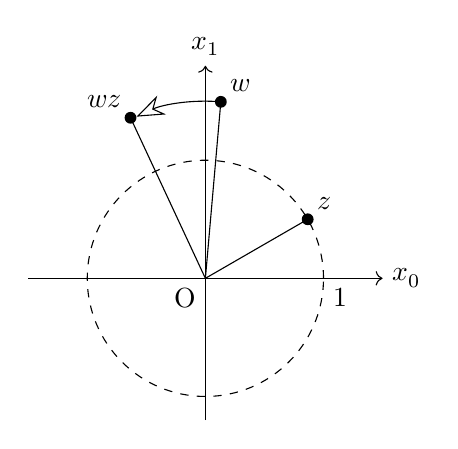
\begin{tikzpicture}[scale=1.5]
        % 座標軸
        \draw[->] (-1.5,0)--(1.5,0) node[right]{\(x_0\)};
        \draw[->] (0,-1.2)--(0,1.8) node[above]{\(x_1\)};
        % 定義
        \coordinate (O) at (0,0);
        \coordinate (Z) at (30:1);
        \coordinate (W) at (85:1.5);
        \coordinate (WZ) at (115:1.5);
        % 単位円
        \draw (O) node[below left]{O};
        \draw[dashed] (O) circle[radius=1];
        \draw (1,0) node[below right]{\(1\)};
        % Z / W / WZ
        \fill (Z) circle[radius=0.05];
        \draw (O)--(Z) node[above right]{\(z\)};
        \fill (W) circle[radius=0.05];
        \draw (O)--(W) node[above right]{\(w\)};
        \fill (WZ) circle[radius=0.05];
        \draw (O)--(WZ) node[above left]{\(wz\)};
        % 回転
        \draw[-{Stealth[fill=none,length=10]}] (W) arc[start angle=85, end angle=115, radius=1.4];
    \end{tikzpicture}
\end{figure}

2次元空間の回転が複素数で表現できるなら、同じように3次元空間の回転を何らかの数で表現できないだろうか、というのが、ハミルトンが複素数の拡張を考えた動機だったようです。
その結果、四元数にたどり着きました。

3次元空間上の点の回転は、実は四元数を使って次のように表現できます。
四元数の実部を除いた純虚四元数 \(x=x_1\ii+x_2\jj+x_3\kk\) を考えます。
それを3次元空間の点 \(x=(x_1,x_2,x_3)\) と対応させることにします。
3次元空間の点 \(x\) を回転する操作は、純虚四元数 \(x\) に対して大きさ \(1\) の四元数 \(q\) を使った次の操作
\[
    x\mapsto qxq^{-1}
\]
として表現できます。

今回の講演では、この四元数と3次元空間の回転について説明します。
前提知識としては、複素数、三角関数(特に加法定理)、行列(2〜3次)の計算ができれば十分と想定しています。

\end{document}
